\documentclass[aspectratio=169]{beamer}
\usetheme{Madrid}
\usecolortheme{whale}

\usepackage[utf8]{inputenc}
\usepackage[T1]{fontenc}
\usepackage{graphicx}
\usepackage{amsmath}
\usepackage{amssymb}
\usepackage{booktabs}
\usepackage{algorithm}
\usepackage{algorithmic}
\usepackage{tikz}
\usetikzlibrary{shapes,arrows,positioning,fit,calc}
\usepackage{listings}
\usepackage{xcolor}
\usepackage{subcaption}

% Code listing style
\lstset{
    basicstyle=\tiny\ttfamily,
    keywordstyle=\color{blue},
    commentstyle=\color{green!60!black},
    stringstyle=\color{red},
    numbers=left,
    numberstyle=\tiny,
    frame=single,
    breaklines=true
}

\title[Image Restoration Pipeline]{Adaptive Multi-Stage Image Restoration Pipeline}
\subtitle{CE 490 - Image Processing Project}
\author{Image Processing Team}
\institute{Computer Engineering Department}
\date{\today}

\begin{document}

%==============================================================================
% TITLE SLIDE
%==============================================================================
\begin{frame}
    \titlepage
\end{frame}

%==============================================================================
% OUTLINE
%==============================================================================
\begin{frame}{Outline}
    \tableofcontents
\end{frame}

%==============================================================================
% SECTION 1: PROBLEM DISCOVERY
%==============================================================================
\section{Problem Discovery \& Analysis}

\begin{frame}{Problem Statement}
    \begin{block}{Challenge}
        Images degraded by \textbf{mixed noise types}:
        \begin{itemize}
            \item \textbf{Salt \& Pepper Noise} - Impulse noise causing extreme pixel values (0 or 255)
            \item \textbf{Gaussian Noise} - Additive white noise affecting all pixels
            \item \textbf{Edge Degradation} - Loss of sharpness and fine details
        \end{itemize}
    \end{block}
    
    \begin{alertblock}{Goal}
        Restore degraded images while:
        \begin{itemize}
            \item Removing salt \& pepper noise
            \item Reducing Gaussian noise
            \item Preserving and enhancing edges
            \item Maximizing PSNR, SSIM metrics
        \end{itemize}
    \end{alertblock}
\end{frame}

\begin{frame}{Test Images Dataset}
    \begin{columns}
        \column{0.5\textwidth}
        \textbf{Standard Test Images:}
        \begin{itemize}
            \item Boat
            \item Baboon
            \item Barbara
            \item Peppers
            \item Cameraman
        \end{itemize}
        
        \column{0.5\textwidth}
        \textbf{Image Properties:}
        \begin{itemize}
            \item Grayscale (8-bit)
            \item Various texture complexities
            \item Different edge characteristics
            \item Standard benchmark images
        \end{itemize}
    \end{columns}
    
    \vspace{0.5cm}
    \begin{block}{Note}
        Each image has both \texttt{clean/original\_*.png} and \texttt{degraded/degraded\_*.png} versions for objective evaluation.
    \end{block}
\end{frame}

\begin{frame}{Degraded Image - Histogram \& FFT Analysis}
    \begin{columns}
        \column{0.5\textwidth}
        \begin{figure}
            \centering
            % \includegraphics[width=0.9\textwidth]{histogram_degraded.png}
            \fbox{\parbox{0.85\textwidth}{\centering\vspace{3cm}\textbf{Histogram}\\(Degraded Image)\vspace{3cm}}}
            \caption{Histogram showing spikes at 0 and 255 (S\&P noise)}
        \end{figure}
        
        \column{0.5\textwidth}
        \begin{figure}
            \centering
            % \includegraphics[width=0.9\textwidth]{fft_degraded.png}
            \fbox{\parbox{0.85\textwidth}{\centering\vspace{3cm}\textbf{FFT Spectrum}\\(Degraded Image)\vspace{3cm}}}
            \caption{FFT showing high-frequency noise content}
        \end{figure}
    \end{columns}
\end{frame}

\begin{frame}{Degraded Image Analysis - Visual}
    \begin{figure}
        \centering
        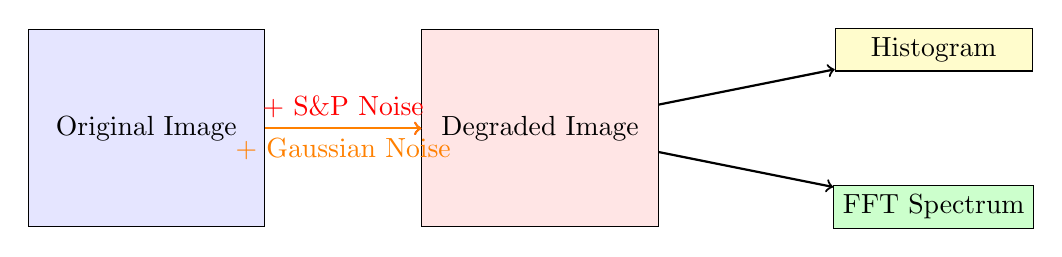
\begin{tikzpicture}
            % Original Image Box
            \node[draw, minimum width=3cm, minimum height=2.5cm, fill=blue!10] (orig) at (0,0) {Original Image};
            
            % Degraded Image Box
            \node[draw, minimum width=3cm, minimum height=2.5cm, fill=red!10] (deg) at (5,0) {Degraded Image};
            
            % Arrow with noise types
            \draw[->, thick, red] (orig) -- (deg) node[midway, above] {+ S\&P Noise};
            \draw[->, thick, orange] (orig) -- (deg) node[midway, below] {+ Gaussian Noise};
            
            % Analysis outputs
            \node[draw, minimum width=2.5cm, fill=yellow!20] (hist) at (10, 1) {Histogram};
            \node[draw, minimum width=2.5cm, fill=green!20] (fft) at (10, -1) {FFT Spectrum};
            
            \draw[->, thick] (deg) -- (hist);
            \draw[->, thick] (deg) -- (fft);
        \end{tikzpicture}
    \end{figure}
    
    \begin{columns}
        \column{0.5\textwidth}
        \textbf{Histogram Analysis:}
        \begin{itemize}
            \item Spikes at 0 and 255 → S\&P noise
            \item Broadened distribution → Gaussian noise
        \end{itemize}
        
        \column{0.5\textwidth}
        \textbf{FFT Analysis:}
        \begin{itemize}
            \item High-frequency content increase
            \item Noise spreads across spectrum
        \end{itemize}
    \end{columns}
\end{frame}

\begin{frame}{Degraded Image Metrics}
    \begin{block}{Quality Metrics (Degraded vs Original)}
        \begin{table}
            \centering
            \begin{tabular}{lccc}
                \toprule
                \textbf{Metric} & \textbf{Definition} & \textbf{Ideal} & \textbf{Degraded (typical)} \\
                \midrule
                MSE & $\frac{1}{MN}\sum(I_{orig} - I_{deg})^2$ & 0 & High \\
                PSNR & $10\log_{10}\frac{255^2}{MSE}$ & $\infty$ dB & 15-25 dB \\
                SSIM & Structural Similarity Index & 1.0 & 0.3-0.7 \\
                \bottomrule
            \end{tabular}
        \end{table}
    \end{block}
    
    \begin{alertblock}{Observed Degradation Characteristics}
        \begin{itemize}
            \item Salt \& Pepper Ratio: $\sim$5-10\% of pixels
            \item Estimated Gaussian Noise $\sigma$: $\sim$10-25
            \item Significant edge blurring and artifact introduction
        \end{itemize}
    \end{alertblock}
\end{frame}

%==============================================================================
% SECTION 2: METRICS AND MEASUREMENT TOOLS
%==============================================================================
\section{Measurement Metrics}

\begin{frame}{Salt \& Pepper Ratio Measurement}
    \begin{block}{Method: Pixel Counting}
        Count pixels with extreme values (0 or 255):
        \begin{equation}
            \text{S\&P Ratio} = \frac{N_{salt} + N_{pepper}}{N_{total}} = \frac{|\{p : p = 0\}| + |\{p : p = 255\}|}{M \times N}
        \end{equation}
    \end{block}
    
    \begin{columns}
        \column{0.5\textwidth}
        \textbf{Algorithm:}
        \begin{enumerate}
            \item Convert image to double
            \item Count pixels = 255 (salt)
            \item Count pixels = 0 (pepper)
            \item Compute ratio
        \end{enumerate}
        
        \column{0.5\textwidth}
        \textbf{Usage in Pipeline:}
        \begin{itemize}
            \item Initial noise estimation
            \item Adaptive Median termination
            \item Threshold: 1\% (0.01)
        \end{itemize}
    \end{columns}
\end{frame}

\begin{frame}{Gaussian Noise Estimation - Laplacian-MAD Method}
    \begin{block}{Principle}
        The Laplacian operator enhances noise while suppressing smooth regions. Using Median Absolute Deviation (MAD) provides robust estimation.
    \end{block}
    
    \begin{equation}
        \sigma_{noise} = \frac{\text{median}(|\nabla^2 I|)}{0.6745 \times \sqrt{20}}
    \end{equation}
    
    \begin{columns}
        \column{0.5\textwidth}
        \textbf{Laplacian Kernel:}
        \begin{equation}
            \nabla^2 = \begin{bmatrix} 0 & 1 & 0 \\ 1 & -4 & 1 \\ 0 & 1 & 0 \end{bmatrix}
        \end{equation}
        
        \column{0.5\textwidth}
        \textbf{MAD Formula:}
        \begin{equation}
            \text{MAD} = \text{median}(|X - \text{median}(X)|)
        \end{equation}
        For Gaussian: $\sigma = \text{MAD} / 0.6745$
    \end{columns}
    
    \vspace{0.3cm}
    \small{Reference: Donoho, D.L. (1995). "De-noising by soft-thresholding", IEEE Trans. Information Theory}
\end{frame}

\begin{frame}{Edge-Noise Metrics}
    \begin{block}{Dual Metric System}
        Simultaneously measure edge strength and noise level in flat regions.
    \end{block}
    
    \begin{columns}
        \column{0.5\textwidth}
        \textbf{Edge Strength (Tenengrad-like):}
        \begin{equation}
            E = \frac{1}{MN}\sum \sqrt{G_x^2 + G_y^2}
        \end{equation}
        where $G_x, G_y$ are Sobel gradients
        
        \column{0.5\textwidth}
        \textbf{Flat-Region Noise:}
        \begin{equation}
            N_{flat} = \text{std}(\nabla^2 I |_{flat})
        \end{equation}
        Flat mask: bottom 30\% of gradient magnitudes
    \end{columns}
    
    \vspace{0.3cm}
    \begin{alertblock}{Key Insight}
        This dual metric allows balancing edge enhancement vs. noise amplification in sharpening steps.
    \end{alertblock}
\end{frame}

\begin{frame}{Standard Quality Metrics}
    \begin{columns}
        \column{0.33\textwidth}
        \textbf{MSE}
        \begin{equation}
            \text{MSE} = \frac{1}{MN}\sum_{i,j}(I_o - I_r)^2
        \end{equation}
        \begin{itemize}
            \item Lower is better
            \item Normalized [0,1]
        \end{itemize}
        
        \column{0.33\textwidth}
        \textbf{PSNR}
        \begin{equation}
            \text{PSNR} = 10\log_{10}\frac{1}{\text{MSE}}
        \end{equation}
        \begin{itemize}
            \item Higher is better
            \item Typical: 25-40 dB
        \end{itemize}
        
        \column{0.33\textwidth}
        \textbf{SSIM}
        \begin{equation}
            \text{SSIM} = f(l, c, s)
        \end{equation}
        \begin{itemize}
            \item Range: [-1, 1]
            \item 1 = identical
        \end{itemize}
    \end{columns}
    
    \vspace{0.5cm}
    \begin{block}{SSIM Components}
        \begin{itemize}
            \item \textbf{Luminance} ($l$): Mean intensity comparison
            \item \textbf{Contrast} ($c$): Standard deviation comparison
            \item \textbf{Structure} ($s$): Normalized cross-correlation
        \end{itemize}
    \end{block}
\end{frame}

%==============================================================================
% SECTION 3: PIPELINE OVERVIEW
%==============================================================================
\section{Pipeline Overview}

\begin{frame}{Complete Pipeline Architecture}
    \begin{figure}
        \centering
        \resizebox{\textwidth}{!}{
        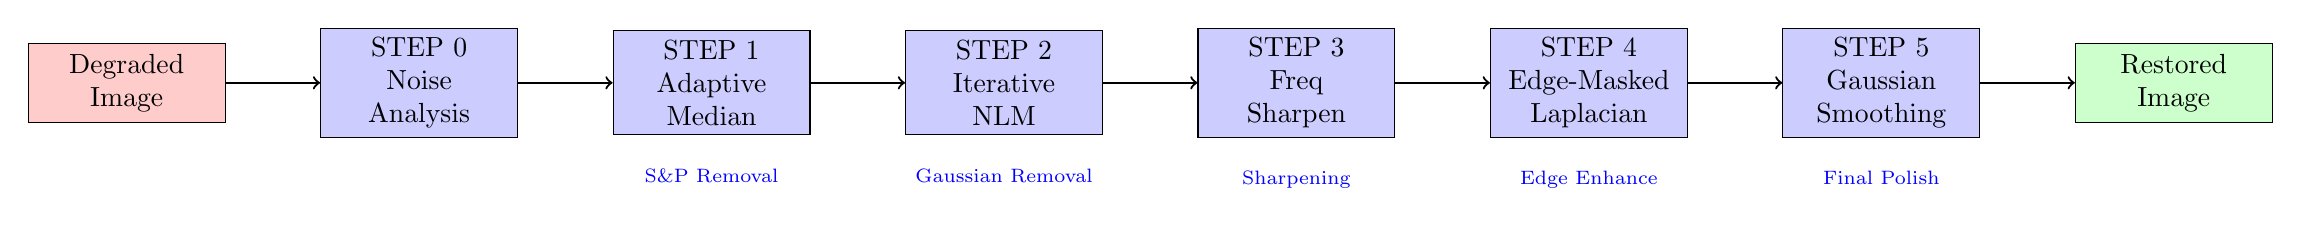
\begin{tikzpicture}[
            node distance=1.2cm,
            block/.style={rectangle, draw, fill=blue!20, minimum width=2.5cm, minimum height=1cm, align=center},
            decision/.style={diamond, draw, fill=yellow!20, minimum width=1.5cm, align=center, aspect=2},
            arrow/.style={->, thick}
        ]
            % Nodes
            \node[block, fill=red!20] (input) {Degraded\\Image};
            \node[block, right=of input] (step0) {STEP 0\\Noise\\Analysis};
            \node[block, right=of step0] (step1) {STEP 1\\Adaptive\\Median};
            \node[block, right=of step1] (step2) {STEP 2\\Iterative\\NLM};
            \node[block, right=of step2] (step3) {STEP 3\\Freq\\Sharpen};
            \node[block, right=of step3] (step4) {STEP 4\\Edge-Masked\\Laplacian};
            \node[block, right=of step4] (step5) {STEP 5\\Gaussian\\Smoothing};
            \node[block, fill=green!20, right=of step5] (output) {Restored\\Image};
            
            % Arrows
            \draw[arrow] (input) -- (step0);
            \draw[arrow] (step0) -- (step1);
            \draw[arrow] (step1) -- (step2);
            \draw[arrow] (step2) -- (step3);
            \draw[arrow] (step3) -- (step4);
            \draw[arrow] (step4) -- (step5);
            \draw[arrow] (step5) -- (output);
            
            % Labels below
            \node[below=0.3cm of step1, text=blue, font=\scriptsize] {S\&P Removal};
            \node[below=0.3cm of step2, text=blue, font=\scriptsize] {Gaussian Removal};
            \node[below=0.3cm of step3, text=blue, font=\scriptsize] {Sharpening};
            \node[below=0.3cm of step4, text=blue, font=\scriptsize] {Edge Enhance};
            \node[below=0.3cm of step5, text=blue, font=\scriptsize] {Final Polish};
        \end{tikzpicture}
        }
    \end{figure}
    
    \begin{block}{Pipeline Philosophy}
        \begin{itemize}
            \item \textbf{Progressive}: Each step builds on previous results
            \item \textbf{Adaptive}: Parameters tuned per-image using grid search
            \item \textbf{Iterative}: Steps repeat until convergence criteria met
            \item \textbf{Metric-Driven}: Decisions based on quantitative measurements
        \end{itemize}
    \end{block}
\end{frame}

\begin{frame}{Pipeline Design Principles}
    \begin{columns}
        \column{0.5\textwidth}
        \textbf{Order Rationale:}
        \begin{enumerate}
            \item \textbf{S\&P First}: Impulse noise must be removed before any smoothing/filtering
            \item \textbf{Then Gaussian}: NLM works best on clean (non-impulse) images
            \item \textbf{Then Sharpen}: Restore edges lost during denoising
            \item \textbf{Edge Enhancement}: Targeted improvement using detected edges
            \item \textbf{Final Polish}: Light smoothing to remove residual artifacts
        \end{enumerate}
        
        \column{0.5\textwidth}
        \textbf{Key Features:}
        \begin{itemize}
            \item \textbf{Iterative Processing}: Steps repeat until threshold reached
            \item \textbf{Grid Search}: Optimal parameters found automatically
            \item \textbf{Early Stopping}: Prevents over-processing
            \item \textbf{Edge Preservation}: Monitored throughout pipeline
        \end{itemize}
    \end{columns}
\end{frame}

%==============================================================================
% SECTION 4: STEP-BY-STEP EXPLANATION
%==============================================================================
\section{Pipeline Steps - Detailed}

\subsection{Step 0: Noise Analysis}

\begin{frame}{Step 0: Initial Noise Analysis}
    \begin{block}{Purpose}
        Characterize the noise in degraded image before processing.
    \end{block}
    
    \begin{columns}
        \column{0.5\textwidth}
        \textbf{Estimated Values (Blind):}
        \begin{itemize}
            \item S\&P Ratio: Count 0/255 pixels
            \item Gaussian $\sigma$: Laplacian-MAD method
        \end{itemize}
        
        \textbf{True Values (Reference):}
        \begin{itemize}
            \item Compare with original
            \item S\&P: Changed pixels that are 0/255
            \item Gaussian: Std of non-S\&P differences
        \end{itemize}
        
        \column{0.5\textwidth}
        \textbf{Computed Metrics:}
        \begin{equation}
            \text{MSE}_0 = \frac{1}{MN}\sum(O - D)^2
        \end{equation}
        \begin{equation}
            \text{PSNR}_0 = 10\log_{10}\frac{255^2}{\text{MSE}_0}
        \end{equation}
        \begin{equation}
            \text{SSIM}_0 = \text{ssim}(D, O)
        \end{equation}
    \end{columns}
    
    \vspace{0.3cm}
    \begin{alertblock}{Output}
        Baseline metrics for comparison and initial parameters for subsequent steps.
    \end{alertblock}
\end{frame}

\subsection{Step 1: Adaptive Median Filter}

\begin{frame}{Step 1: Iterative Adaptive Median Filter}
    \begin{block}{Goal}
        Remove salt \& pepper noise while preserving edges better than standard median filter.
    \end{block}
    
    \textbf{Algorithm - Two-Level Decision:}
    
    \begin{columns}
        \column{0.5\textwidth}
        \textbf{Level A:} Is median an impulse?
        \begin{equation}
            A_1 = z_{med} - z_{min} > 0
        \end{equation}
        \begin{equation}
            A_2 = z_{med} - z_{max} < 0
        \end{equation}
        If both true → Go to Level B\\
        Else → Increase window size
        
        \column{0.5\textwidth}
        \textbf{Level B:} Is original pixel an impulse?
        \begin{equation}
            B_1 = z_{xy} - z_{min} > 0
        \end{equation}
        \begin{equation}
            B_2 = z_{xy} - z_{max} < 0
        \end{equation}
        If both true → Keep $z_{xy}$\\
        Else → Replace with $z_{med}$
    \end{columns}
\end{frame}

\begin{frame}{Step 1: Adaptive Median - Iterative Process}
    \begin{figure}
        \centering
        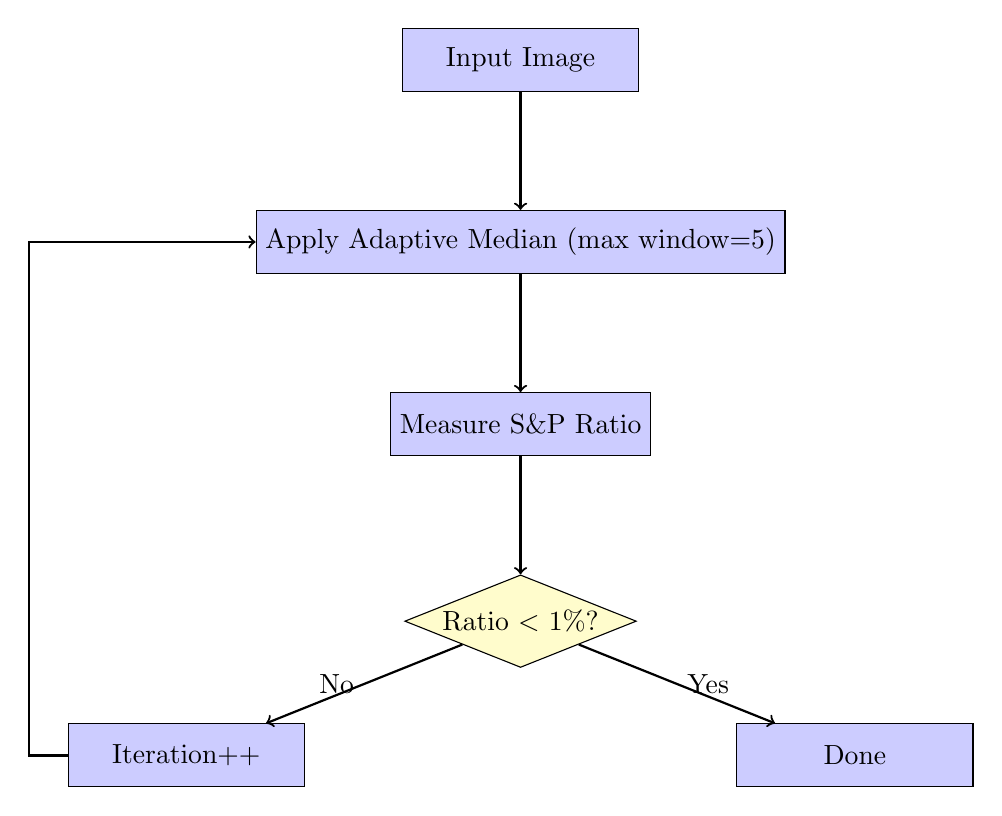
\begin{tikzpicture}[
            node distance=1.5cm,
            block/.style={rectangle, draw, fill=blue!20, minimum width=3cm, minimum height=0.8cm},
            decision/.style={diamond, draw, fill=yellow!20, aspect=2.5, inner sep=1pt},
            arrow/.style={->, thick}
        ]
            \node[block] (start) {Input Image};
            \node[block, below=of start] (amf) {Apply Adaptive Median (max window=5)};
            \node[block, below=of amf] (measure) {Measure S\&P Ratio};
            \node[decision, below=of measure] (check) {Ratio $<$ 1\%?};
            \node[block, below left=1cm and 2cm of check] (continue) {Iteration++};
            \node[block, below right=1cm and 2cm of check] (done) {Done};
            
            \draw[arrow] (start) -- (amf);
            \draw[arrow] (amf) -- (measure);
            \draw[arrow] (measure) -- (check);
            \draw[arrow] (check) -- node[left] {No} (continue);
            \draw[arrow] (check) -- node[right] {Yes} (done);
            \draw[arrow] (continue) -- +(-2,0) |- (amf);
        \end{tikzpicture}
    \end{figure}
    
    \begin{block}{Parameters}
        \begin{itemize}
            \item \textbf{Max Window Size}: 5×5
            \item \textbf{Threshold}: S\&P Ratio $<$ 0.01 (1\%)
            \item \textbf{Max Iterations}: 10
        \end{itemize}
    \end{block}
\end{frame}

\begin{frame}{Step 1: Adaptive Median - Window Growth}
    \begin{figure}
        \centering
        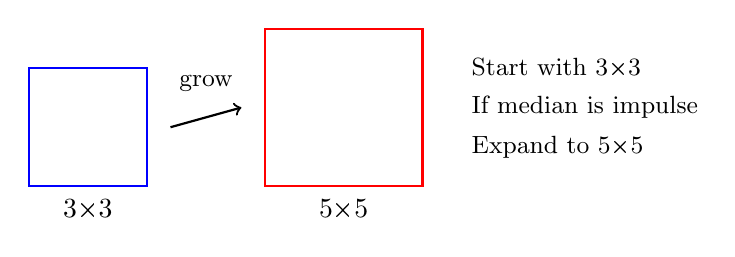
\begin{tikzpicture}
            % 3x3 window
            \draw[thick, blue] (0,0) rectangle (1.5,1.5);
            \node at (0.75, -0.3) {3×3};
            
            % 5x5 window
            \draw[thick, red] (3,0) rectangle (5,2);
            \node at (4, -0.3) {5×5};
            
            % Arrow
            \draw[->, thick] (1.8, 0.75) -- (2.7, 1);
            \node at (2.25, 1.3) {\small grow};
            
            % Labels
            \node[right] at (5.5, 1.5) {\small Start with 3×3};
            \node[right] at (5.5, 1) {\small If median is impulse};
            \node[right] at (5.5, 0.5) {\small Expand to 5×5};
        \end{tikzpicture}
    \end{figure}
    
    \begin{block}{Advantage over Standard Median}
        \begin{itemize}
            \item \textbf{Adaptive window}: Smaller windows preserve edges, larger windows handle dense noise
            \item \textbf{Impulse detection}: Only replaces actual noise pixels
            \item \textbf{Edge preservation}: Clean pixels kept unchanged
        \end{itemize}
    \end{block}
\end{frame}

\begin{frame}{Step 1: Results}
    \begin{columns}
        \column{0.5\textwidth}
        \begin{block}{Metrics After Step 1}
            \begin{table}
                \centering
                \begin{tabular}{lc}
                    \toprule
                    \textbf{Metric} & \textbf{Value} \\
                    \midrule
                    MSE & \textit{[Insert Value]} \\
                    PSNR (dB) & \textit{[Insert Value]} \\
                    SSIM & \textit{[Insert Value]} \\
                    S\&P Ratio & \textit{[Insert Value]} \\
                    Iterations & \textit{[Insert Value]} \\
                    \bottomrule
                \end{tabular}
            \end{table}
        \end{block}
        
        \column{0.5\textwidth}
        \begin{figure}
            \centering
            % \includegraphics[width=\textwidth]{step1_result.png}
            \fbox{\parbox{0.9\textwidth}{\centering\vspace{2cm}Step 1 Result Image\\(Adaptive Median Output)\vspace{2cm}}}
            \caption{After Adaptive Median Filter}
        \end{figure}
    \end{columns}
\end{frame}

\subsection{Step 2: Non-Local Means}

\begin{frame}{Step 2: Iterative Non-Local Means (NLM)}
    \begin{block}{Goal}
        Remove Gaussian noise while preserving texture and fine details.
    \end{block}
    
    \textbf{NLM Principle:}
    \begin{equation}
        \hat{I}(p) = \sum_{q \in S} w(p,q) \cdot I(q)
    \end{equation}
    
    \begin{equation}
        w(p,q) = \frac{1}{Z(p)} \exp\left(-\frac{\|N(p) - N(q)\|^2}{h^2}\right)
    \end{equation}
    
    \begin{itemize}
        \item $N(p)$: Neighborhood (patch) around pixel $p$
        \item $S$: Search window
        \item $h$: Degree of smoothing (filtering parameter)
        \item $Z(p)$: Normalization factor
    \end{itemize}
\end{frame}

\begin{frame}{Step 2: NLM - Grid Search Parameters}
    \begin{block}{Parameter Space}
        \begin{table}
            \centering
            \begin{tabular}{ll}
                \toprule
                \textbf{Parameter} & \textbf{Values} \\
                \midrule
                Degree of Smoothing & [5, 10, 15, 20, 30] \\
                Search Window Size & [11, 21] (odd) \\
                Comparison Window Size & [3, 5, 7] (odd) \\
                \bottomrule
            \end{tabular}
        \end{table}
    \end{block}
    
    \begin{columns}
        \column{0.5\textwidth}
        \textbf{Selection Criterion:}
        \begin{itemize}
            \item Minimize estimated Gaussian noise
            \item Laplacian-MAD measurement
            \item Early stopping if no improvement
        \end{itemize}
        
        \column{0.5\textwidth}
        \textbf{Stopping Conditions:}
        \begin{itemize}
            \item Gaussian noise $<$ 0.1
            \item Max iterations: 5
            \item No improvement found
        \end{itemize}
    \end{columns}
\end{frame}

\begin{frame}{Step 2: NLM - Iterative Flow}
    \begin{figure}
        \centering
        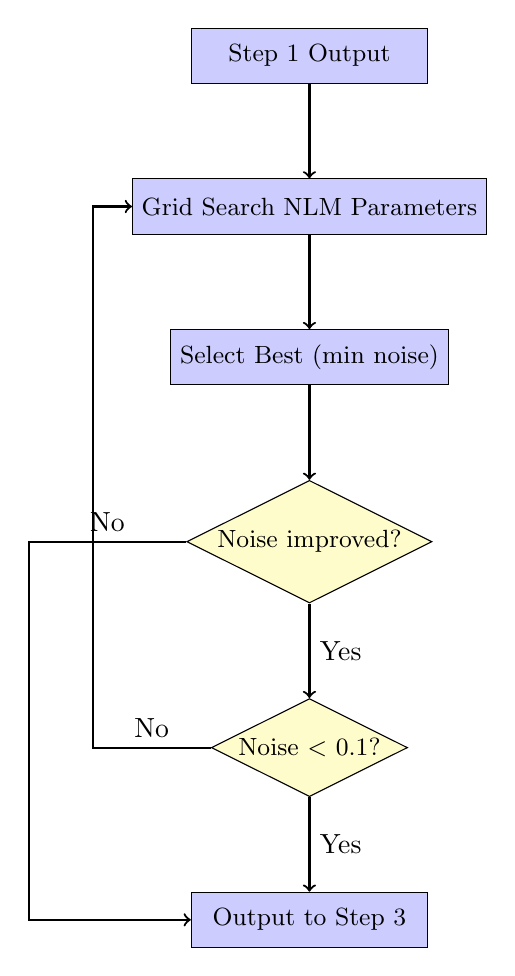
\begin{tikzpicture}[
            node distance=1.2cm,
            block/.style={rectangle, draw, fill=blue!20, minimum width=3cm, minimum height=0.7cm, font=\small},
            decision/.style={diamond, draw, fill=yellow!20, aspect=2, inner sep=1pt, font=\small},
            arrow/.style={->, thick}
        ]
            \node[block] (input) {Step 1 Output};
            \node[block, below=of input] (grid) {Grid Search NLM Parameters};
            \node[block, below=of grid] (select) {Select Best (min noise)};
            \node[decision, below=of select] (improve) {Noise improved?};
            \node[decision, below=of improve] (thresh) {Noise $<$ 0.1?};
            \node[block, below=of thresh] (output) {Output to Step 3};
            
            \draw[arrow] (input) -- (grid);
            \draw[arrow] (grid) -- (select);
            \draw[arrow] (select) -- (improve);
            \draw[arrow] (improve) -- node[right] {Yes} (thresh);
            \draw[arrow] (improve.west) -- node[above] {No} ++(-2,0) |- (output);
            \draw[arrow] (thresh) -- node[right] {Yes} (output);
            \draw[arrow] (thresh.west) -- node[above] {No} ++(-1.5,0) |- (grid);
        \end{tikzpicture}
    \end{figure}
\end{frame}

\begin{frame}{Step 2: Results}
    \begin{columns}
        \column{0.5\textwidth}
        \begin{block}{Metrics After Step 2}
            \begin{table}
                \centering
                \begin{tabular}{lc}
                    \toprule
                    \textbf{Metric} & \textbf{Value} \\
                    \midrule
                    MSE & \textit{[Insert Value]} \\
                    PSNR (dB) & \textit{[Insert Value]} \\
                    SSIM & \textit{[Insert Value]} \\
                    Gaussian $\sigma$ & \textit{[Insert Value]} \\
                    Iterations & \textit{[Insert Value]} \\
                    Best Params & \textit{[deg, SW, CW]} \\
                    \bottomrule
                \end{tabular}
            \end{table}
        \end{block}
        
        \column{0.5\textwidth}
        \begin{figure}
            \centering
            % \includegraphics[width=\textwidth]{step2_result.png}
            \fbox{\parbox{0.9\textwidth}{\centering\vspace{2cm}Step 2 Result Image\\(NLM Output)\vspace{2cm}}}
            \caption{After Non-Local Means}
        \end{figure}
    \end{columns}
\end{frame}

\subsection{Step 3: Frequency Domain Sharpening}

\begin{frame}{Step 3: Iterative Frequency High-Boost Sharpening}
    \begin{block}{Goal}
        Restore edges lost during denoising using frequency-domain filtering.
    \end{block}
    
    \textbf{High-Boost Filter:}
    \begin{equation}
        G(u,v) = 1 + k \cdot H_{HP}(u,v)
    \end{equation}
    
    \textbf{Gaussian High-Pass:}
    \begin{equation}
        H_{HP}(u,v) = 1 - H_{LP}(u,v) = 1 - e^{-\frac{D(u,v)^2}{2\sigma_c^2}}
    \end{equation}
    
    where $D(u,v) = \sqrt{u^2 + v^2}$ is the distance from center.
    
    \begin{block}{Parameters}
        \begin{itemize}
            \item $k$: Boost strength [0.3, 0.5, 0.7, 0.9, 1.1, 1.3, 1.5, 1.8, 2.0]
            \item $\sigma_c$: Cutoff frequency [0.03, 0.05, 0.07, 0.09, 0.11, 0.13]
        \end{itemize}
    \end{block}
\end{frame}

\begin{frame}{Step 3: Sharpening - Selection Criterion}
    \begin{block}{Edge vs Noise Trade-off}
        \begin{equation}
            \text{ratio} = \frac{\text{noise\_gain}}{\text{edge\_gain}}
        \end{equation}
        
        \begin{itemize}
            \item \textbf{edge\_gain} = $\frac{E_{new}}{E_{old}} - 1$ (how much edge increased)
            \item \textbf{noise\_gain} = $\frac{N_{new}}{N_{old}} - 1$ (how much noise increased)
            \item \textbf{Select}: Parameter with \textbf{lowest ratio} (max edge, min noise)
        \end{itemize}
    \end{block}
    
    \begin{alertblock}{Early Stopping Conditions}
        \begin{enumerate}
            \item Ratio $\geq$ 3.0 (noise increasing too fast)
            \item Noise level $>$ 0.03 (absolute threshold)
            \item Max iterations: 5
        \end{enumerate}
    \end{alertblock}
\end{frame}

\begin{frame}{Step 3: Frequency Domain Visualization}
    \begin{figure}
        \centering
        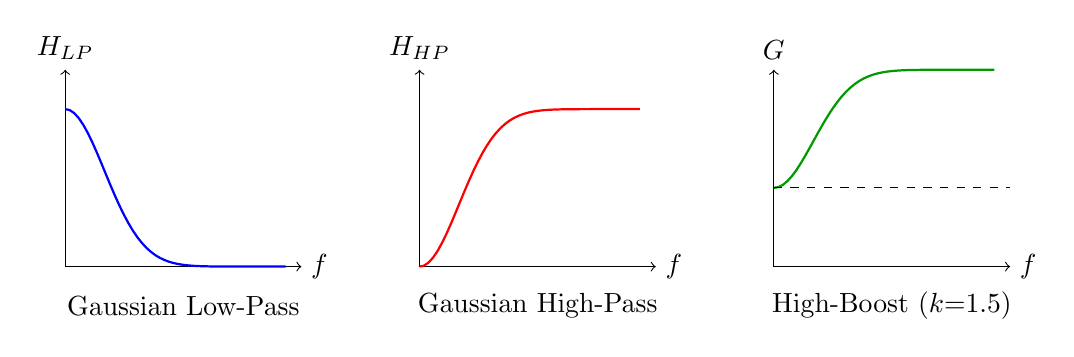
\begin{tikzpicture}
            % Low-pass response
            \begin{scope}[shift={(0,0)}]
                \draw[->] (0,0) -- (3,0) node[right] {$f$};
                \draw[->] (0,0) -- (0,2.5) node[above] {$H_{LP}$};
                \draw[thick, blue, domain=0:2.8, samples=50] plot (\x, {2*exp(-\x*\x/0.5)});
                \node at (1.5, -0.5) {Gaussian Low-Pass};
            \end{scope}
            
            % High-pass response
            \begin{scope}[shift={(4.5,0)}]
                \draw[->] (0,0) -- (3,0) node[right] {$f$};
                \draw[->] (0,0) -- (0,2.5) node[above] {$H_{HP}$};
                \draw[thick, red, domain=0:2.8, samples=50] plot (\x, {2*(1-exp(-\x*\x/0.5))});
                \node at (1.5, -0.5) {Gaussian High-Pass};
            \end{scope}
            
            % High-boost response
            \begin{scope}[shift={(9,0)}]
                \draw[->] (0,0) -- (3,0) node[right] {$f$};
                \draw[->] (0,0) -- (0,2.5) node[above] {$G$};
                \draw[thick, green!60!black, domain=0:2.8, samples=50] plot (\x, {1 + 1.5*(1-exp(-\x*\x/0.5))});
                \draw[dashed] (0,1) -- (3,1);
                \node at (1.5, -0.5) {High-Boost ($k$=1.5)};
            \end{scope}
        \end{tikzpicture}
    \end{figure}
    
    \begin{block}{Process}
        \begin{enumerate}
            \item FFT of image → Frequency domain
            \item Multiply by high-boost filter $G(u,v)$
            \item Inverse FFT → Enhanced image
        \end{enumerate}
    \end{block}
\end{frame}

\begin{frame}{Step 3: Results}
    \begin{columns}
        \column{0.5\textwidth}
        \begin{block}{Metrics After Step 3}
            \begin{table}
                \centering
                \begin{tabular}{lc}
                    \toprule
                    \textbf{Metric} & \textbf{Value} \\
                    \midrule
                    Edge Strength & \textit{[Insert Value]} \\
                    Noise (flat) & \textit{[Insert Value]} \\
                    Iterations & \textit{[Insert Value]} \\
                    Best $k$ & \textit{[Insert Value]} \\
                    Best cutoff & \textit{[Insert Value]} \\
                    \bottomrule
                \end{tabular}
            \end{table}
        \end{block}
        
        \column{0.5\textwidth}
        \begin{figure}
            \centering
            % \includegraphics[width=\textwidth]{step3_result.png}
            \fbox{\parbox{0.9\textwidth}{\centering\vspace{2cm}Step 3 Result Image\\(Freq Sharpen Output)\vspace{2cm}}}
            \caption{After Frequency Sharpening}
        \end{figure}
    \end{columns}
\end{frame}

\subsection{Step 4: Laplacian Enhancement}

\begin{frame}{Step 4: Laplacian Enhancement}
    \begin{block}{Goal}
        Enhance edges using Laplacian filtering on sharpened image (Step 3) and combine with NLM output.
    \end{block}
    
    \textbf{Process:}
    \begin{enumerate}
        \item Compute Laplacian of sharpened image (Step 3)
        \item Apply Wiener filter to reduce noise (using estimated variance)
        \item Apply light mean filter (3×3) for smoothing
        \item Add processed Laplacian to Step 2 (NLM) output
    \end{enumerate}
    
    \begin{equation}
        I_{final} = I_{NLM} + \text{mean}(\text{wiener}(\nabla^2 I_{sharp}))
    \end{equation}
\end{frame}

\begin{frame}{Step 4: Laplacian Enhancement - Flow}
    \begin{figure}
        \centering
        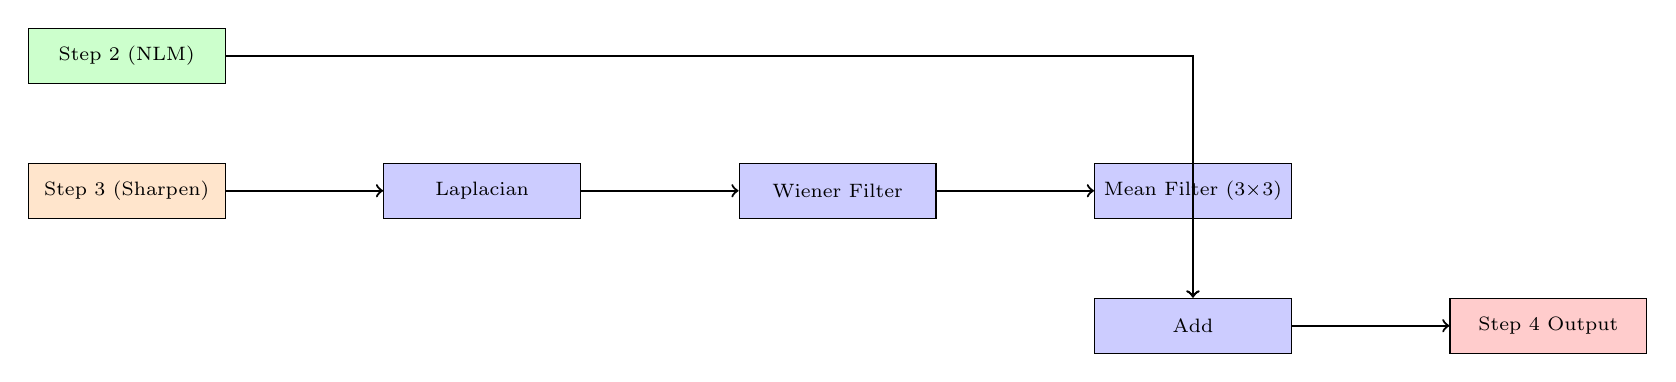
\begin{tikzpicture}[
            node distance=1cm and 2cm,
            block/.style={rectangle, draw, fill=blue!20, minimum width=2.5cm, minimum height=0.7cm, font=\scriptsize},
            arrow/.style={->, thick}
        ]
            % Input nodes
            \node[block, fill=green!20] (step2) {Step 2 (NLM)};
            \node[block, fill=orange!20, below=of step2] (step3) {Step 3 (Sharpen)};
            
            % Processing
            \node[block, right=of step3] (laplace) {Laplacian};
            \node[block, right=of laplace] (wiener) {Wiener Filter};
            \node[block, right=of wiener] (mean) {Mean Filter (3×3)};
            
            % Output
            \node[block, below=of mean] (add) {Add};
            \node[block, fill=red!20, right=of add] (output) {Step 4 Output};
            
            % Arrows
            \draw[arrow] (step3) -- (laplace);
            \draw[arrow] (laplace) -- (wiener);
            \draw[arrow] (wiener) -- (mean);
            \draw[arrow] (mean) -- (add);
            \draw[arrow] (step2) -| (add);
            \draw[arrow] (add) -- (output);
        \end{tikzpicture}
    \end{figure}
    
    \begin{block}{Key Components}
        \begin{itemize}
            \item \textbf{Laplacian}: Second-order derivative for edge enhancement
            \item \textbf{Wiener Filter}: Reduces noise using estimated variance from edge\_noise\_metrics
            \item \textbf{Mean Filter}: 3×3 light smoothing for artifact removal
        \end{itemize}
    \end{block}
\end{frame}

\begin{frame}{Step 4: Laplacian Kernel \& Noise Reduction}
    \begin{columns}
        \column{0.5\textwidth}
        \textbf{Laplacian Kernel (4-connected):}
        \begin{equation}
            \nabla^2 = \begin{bmatrix} 0 & -1 & 0 \\ -1 & 4 & -1 \\ 0 & -1 & 0 \end{bmatrix}
        \end{equation}
        
        \textbf{Properties:}
        \begin{itemize}
            \item Second-order derivative
            \item Enhances edges in all directions
            \item Zero response on constant regions
        \end{itemize}
        
        \column{0.5\textwidth}
        \textbf{Noise Reduction Strategy:}
        \begin{itemize}
            \item Wiener filter with estimated noise variance
            \item Variance from edge\_noise\_metrics: $\sigma^2$
            \item Light mean filter (3×3) for final smoothing
            \item Combines edge enhancement with noise control
        \end{itemize}
    \end{columns}
\end{frame}

\begin{frame}{Step 4: Results}
    \begin{columns}
        \column{0.5\textwidth}
        \begin{block}{Metrics After Step 4}
            \begin{table}
                \centering
                \begin{tabular}{lc}
                    \toprule
                    \textbf{Metric} & \textbf{Value} \\
                    \midrule
                    MSE & \textit{[Insert Value]} \\
                    PSNR (dB) & \textit{[Insert Value]} \\
                    SSIM & \textit{[Insert Value]} \\
                    \bottomrule
                \end{tabular}
            \end{table}
        \end{block}
        
        \column{0.5\textwidth}
        \begin{figure}
            \centering
            % \includegraphics[width=\textwidth]{step4_result.png}
            \fbox{\parbox{0.9\textwidth}{\centering\vspace{2cm}Step 4 Result Image\\(Laplacian Enhancement Output)\vspace{2cm}}}
            \caption{After Laplacian Enhancement}
        \end{figure}
    \end{columns}
\end{frame}

\subsection{Step 5: Gaussian Smoothing}

\begin{frame}{Step 5: Iterative Gaussian Smoothing}
    \begin{block}{Goal}
        Final polish: Remove residual artifacts while strictly preserving edges.
    \end{block}
    
    \textbf{Gaussian Filter:}
    \begin{equation}
        G(x,y) = \frac{1}{2\pi\sigma^2} e^{-\frac{x^2 + y^2}{2\sigma^2}}
    \end{equation}
    
    \begin{block}{Parameters Grid}
        \begin{itemize}
            \item $\sigma$: [0.01, 0.05, 0.1, 0.2, 0.3, 0.4, 0.5, 0.6, 0.8, 1.0]
            \item Filter Size: [3, 5, 7, 9, 11, 13]
        \end{itemize}
    \end{block}
\end{frame}

\begin{frame}{Step 5: Gaussian - Selection Criterion}
    \begin{block}{Edge Preservation Priority}
        \begin{equation}
            \text{ratio} = \frac{\text{noise\_reduction}}{\text{edge\_loss}}
        \end{equation}
        
        Select parameter with \textbf{highest ratio} (max noise reduction per edge loss).
    \end{block}
    
    \begin{alertblock}{Strict Edge Preservation}
        \begin{itemize}
            \item \textbf{Total edge loss} must remain $<$ 10\% from initial
            \item Only apply if noise actually decreases
            \item Early stopping when no valid parameters found
        \end{itemize}
    \end{alertblock}
    
    \begin{block}{Stopping Conditions}
        \begin{enumerate}
            \item No parameter satisfies edge loss $<$ 10\%
            \item Noise not improving
            \item Max iterations: 5
        \end{enumerate}
    \end{block}
\end{frame}

\begin{frame}{Step 5: Results}
    \begin{columns}
        \column{0.5\textwidth}
        \begin{block}{Metrics After Step 5}
            \begin{table}
                \centering
                \begin{tabular}{lc}
                    \toprule
                    \textbf{Metric} & \textbf{Value} \\
                    \midrule
                    MSE & \textit{[Insert Value]} \\
                    PSNR (dB) & \textit{[Insert Value]} \\
                    SSIM & \textit{[Insert Value]} \\
                    Edge Strength & \textit{[Insert Value]} \\
                    Noise (flat) & \textit{[Insert Value]} \\
                    Iterations & \textit{[Insert Value]} \\
                    Best $\sigma$ & \textit{[Insert Value]} \\
                    \bottomrule
                \end{tabular}
            \end{table}
        \end{block}
        
        \column{0.5\textwidth}
        \begin{figure}
            \centering
            % \includegraphics[width=\textwidth]{step5_result.png}
            \fbox{\parbox{0.9\textwidth}{\centering\vspace{2cm}Step 5 Result Image\\(Final Gaussian Output)\vspace{2cm}}}
            \caption{After Gaussian Smoothing}
        \end{figure}
    \end{columns}
\end{frame}

%==============================================================================
% SECTION 5: RESULTS
%==============================================================================
\section{Results \& Evaluation}

\begin{frame}{Pipeline Progression - Metrics}
    \begin{block}{Metric Improvement Through Pipeline}
        \begin{table}
            \centering
            \small
            \begin{tabular}{lccc}
                \toprule
                \textbf{Step} & \textbf{MSE} & \textbf{PSNR (dB)} & \textbf{SSIM} \\
                \midrule
                Step 0 (Degraded) & High & Low & Low \\
                Step 1 (Adaptive Median) & $\downarrow\downarrow$ & $\uparrow\uparrow$ & $\uparrow\uparrow$ \\
                Step 2 (NLM) & $\downarrow$ & $\uparrow$ & $\uparrow$ \\
                Step 3 (Sharpen) & $\sim$ & $\sim$ & $\uparrow$ \\
                Step 4 (Edge-Laplacian) & $\sim$ & $\uparrow$ & $\uparrow$ \\
                Step 5 (Gaussian) & $\downarrow$ & $\uparrow$ & $\uparrow$ \\
                \bottomrule
            \end{tabular}
        \end{table}
    \end{block}
    
    \begin{itemize}
        \item \textbf{Biggest improvements}: Steps 1 \& 2 (noise removal)
        \item \textbf{Fine-tuning}: Steps 3, 4, 5 (edge/quality enhancement)
    \end{itemize}
\end{frame}

\begin{frame}{Overall Results Table}
    \begin{block}{Complete Pipeline Metrics Summary}
        \begin{table}
            \centering
            \begin{tabular}{lccc}
                \toprule
                \textbf{Step} & \textbf{MSE} & \textbf{PSNR (dB)} & \textbf{SSIM} \\
                \midrule
                Step 0 (Degraded) & \textit{[Value]} & \textit{[Value]} & \textit{[Value]} \\
                Step 1 (Adaptive Median) & \textit{[Value]} & \textit{[Value]} & \textit{[Value]} \\
                Step 2 (NLM) & \textit{[Value]} & \textit{[Value]} & \textit{[Value]} \\
                Step 4 (Laplacian) & \textit{[Value]} & \textit{[Value]} & \textit{[Value]} \\
                Step 5 (Final) & \textit{[Value]} & \textit{[Value]} & \textit{[Value]} \\
                \midrule
                \textbf{Improvement} & \textit{[\%]} & \textit{[+dB]} & \textit{[+\%]} \\
                \bottomrule
            \end{tabular}
        \end{table}
    \end{block}
    
    \begin{alertblock}{Global Average (All Images)}
        \textbf{MSE}: \textit{[Value]} \quad \textbf{PSNR}: \textit{[Value]} dB \quad \textbf{SSIM}: \textit{[Value]}
    \end{alertblock}
\end{frame}

\begin{frame}{Final Restored Image}
    \begin{figure}
        \centering
        \begin{minipage}{0.45\textwidth}
            \centering
            % \includegraphics[width=\textwidth]{original.png}
            \fbox{\parbox{0.9\textwidth}{\centering\vspace{3cm}Original Image\vspace{3cm}}}
            \caption{Original}
        \end{minipage}
        \hfill
        \begin{minipage}{0.45\textwidth}
            \centering
            % \includegraphics[width=\textwidth]{degraded.png}
            \fbox{\parbox{0.9\textwidth}{\centering\vspace{3cm}Degraded Image\vspace{3cm}}}
            \caption{Degraded}
        \end{minipage}
    \end{figure}
\end{frame}

\begin{frame}{Final Restored Image (cont.)}
    \begin{figure}
        \centering
        \begin{minipage}{0.6\textwidth}
            \centering
            % \includegraphics[width=\textwidth]{final_restored.png}
            \fbox{\parbox{0.95\textwidth}{\centering\vspace{4cm}\textbf{Final Restored Image}\\(Pipeline Output)\vspace{4cm}}}
        \end{minipage}
    \end{figure}
    
    \begin{block}{Final Metrics}
        \centering
        \textbf{MSE}: \textit{[Value]} \quad \textbf{PSNR}: \textit{[Value]} dB \quad \textbf{SSIM}: \textit{[Value]}
    \end{block}
\end{frame}

\begin{frame}{Visual Comparison}
    \begin{block}{Expected Visual Improvements}
        \begin{columns}
            \column{0.5\textwidth}
            \textbf{After Step 1:}
            \begin{itemize}
                \item Salt \& pepper removed
                \item Edges mostly preserved
            \end{itemize}
            
            \textbf{After Step 2:}
            \begin{itemize}
                \item Gaussian noise reduced
                \item Some edge softening
            \end{itemize}
            
            \column{0.5\textwidth}
            \textbf{After Steps 3-4:}
            \begin{itemize}
                \item Edges restored/enhanced
                \item Detail recovery
            \end{itemize}
            
            \textbf{After Step 5:}
            \begin{itemize}
                \item Smooth appearance
                \item Artifact-free result
            \end{itemize}
        \end{columns}
    \end{block}
\end{frame}

\begin{frame}{Edge Quality Assessment}
    \begin{block}{Edge Strength Monitoring}
        Edge\_noise\_metrics tracks edge quality at each stage:
        \begin{itemize}
            \item \textbf{Degraded}: High noise in flat regions, false edge detection
            \item \textbf{After NLM}: Cleaner but potentially weaker edges
            \item \textbf{After Sharpen}: Restored edge strength with controlled noise
            \item \textbf{Final}: Balanced edge preservation with minimal artifacts
        \end{itemize}
    \end{block}
    
    \begin{alertblock}{Key Observation}
        The pipeline successfully removes noise while maintaining or improving edge strength - measured quantitatively throughout the process.
    \end{alertblock}
\end{frame}

%==============================================================================
% SECTION 6: CONCLUSION
%==============================================================================
\section{Conclusion}

\begin{frame}{Summary}
    \begin{block}{Key Contributions}
        \begin{enumerate}
            \item \textbf{Multi-stage pipeline} for mixed noise removal
            \item \textbf{Adaptive parameter selection} via grid search
            \item \textbf{Iterative processing} with convergence criteria
            \item \textbf{Edge-aware processing} throughout pipeline
            \item \textbf{Quantitative metrics} for decision making
        \end{enumerate}
    \end{block}
    
    \begin{block}{Pipeline Strengths}
        \begin{itemize}
            \item Handles both impulse and Gaussian noise
            \item Balances noise removal with edge preservation
            \item Automatic parameter tuning per image
            \item Progressive improvement with early stopping
        \end{itemize}
    \end{block}
\end{frame}

\begin{frame}{Future Work}
    \begin{itemize}
        \item \textbf{Deep Learning Integration}: CNN-based denoising (DnCNN, etc.)
        \item \textbf{Adaptive Thresholds}: Learning optimal thresholds from data
        \item \textbf{Real-time Processing}: GPU acceleration
        \item \textbf{Color Image Support}: Extend to RGB images
        \item \textbf{Blind Deconvolution}: Handle blur in addition to noise
    \end{itemize}
    
    \vspace{0.5cm}
    \begin{block}{Acknowledgments}
        \begin{itemize}
            \item SA-DCT toolbox for advanced filtering options
            \item Standard test images from image processing community
        \end{itemize}
    \end{block}
\end{frame}

\begin{frame}
    \centering
    \Huge Thank You!
    
    \vspace{1cm}
    \Large Questions?
\end{frame}

\end{document}
